\documentclass[runningheads,a4paper]{llncs}

\usepackage[portuguese]{babel}
\usepackage[utf8]{inputenc}
\usepackage{graphicx}

%extended enumerate, such as \begin{compactenum}
\usepackage{paralist}

%put figures inside a text
%\usepackage{picins}
%use
%\piccaptioninside
%\piccaption{...}
%\parpic[r]{\includegraphics ...}
%Text...

%Sorts the citations in the brackets
%\usepackage{cite}

%for easy quotations: \enquote{text}
\usepackage{csquotes}

\usepackage[T1]{fontenc}

%enable margin kerning
\usepackage{microtype}

%better font, similar to the default springer font
\usepackage[%
rm={oldstyle=false,proportional=true},%
sf={oldstyle=false,proportional=true},%
tt={oldstyle=false,proportional=true,variable=true},%
qt=false%
]{cfr-lm}
%
%if more space is needed, exchange cfr-lm by mathptmx
%\usepackage{mathptmx}

%for demonstration purposes only
\usepackage[math]{blindtext}

\usepackage[
%pdfauthor={},
%pdfsubject={},
%pdftitle={},
%pdfkeywords={},
bookmarks=false,
breaklinks=true,
colorlinks=true,
linkcolor=black,
citecolor=black,
urlcolor=black,
%pdfstartpage=19,
pdfpagelayout=SinglePage
]{hyperref}
%enables correct jumping to figures when referencing
\usepackage[all]{hypcap}

\usepackage[capitalise,nameinlink]{cleveref}
%Nice formats for \cref
\crefname{section}{Sect.}{Sect.}
\Crefname{section}{Section}{Sections}
\crefname{figure}{Fig.}{Fig.}
\Crefname{figure}{Figure}{Figures}

\usepackage{xspace}
%\newcommand{\eg}{e.\,g.\xspace}
%\newcommand{\ie}{i.\,e.\xspace}
\newcommand{\eg}{e.\,g.,\ }
\newcommand{\ie}{i.\,e.,\ }

%introduce \powerset - hint by http://matheplanet.com/matheplanet/nuke/html/viewtopic.php?topic=136492&post_id=997377
\DeclareFontFamily{U}{MnSymbolC}{}
\DeclareSymbolFont{MnSyC}{U}{MnSymbolC}{m}{n}
\DeclareFontShape{U}{MnSymbolC}{m}{n}{
    <-6>  MnSymbolC5
   <6-7>  MnSymbolC6
   <7-8>  MnSymbolC7
   <8-9>  MnSymbolC8
   <9-10> MnSymbolC9
  <10-12> MnSymbolC10
  <12->   MnSymbolC12%
}{}
\DeclareMathSymbol{\powerset}{\mathord}{MnSyC}{180}

%improve wrapping of URLs - hint by http://tex.stackexchange.com/a/10419/9075
\makeatletter
\g@addto@macro{\UrlBreaks}{\UrlOrds}
\makeatother

% correct bad hyphenation here
\hyphenation{op-tical net-works semi-conduc-tor}

\begin{document}

%Works on MiKTeX only
%hint by http://goemonx.blogspot.de/2012/01/pdflatex-ligaturen-und-copynpaste.html
%also http://tex.stackexchange.com/questions/4397/make-ligatures-in-linux-libertine-copyable-and-searchable
%This allows a copy'n'paste of the text from the paper
\input glyphtounicode.tex
\pdfgentounicode=1

\title{Controlo de Acessos em Sistemas com Consistência Eventual}
%If Title is too long, use \titlerunning
%\titlerunning{Short Title}

%Single insitute
\author{Tiago Costa, João Leitão, Nuno Preguiça e Albert Linde}

%If there are too many authors, use \authorrunning
%\authorrunning{First Author et al.}
\institute{NOVA LINCS \& DI-FCT-Universidade Nova de Lisboa}

%Multiple insitutes
%Currently disabled
%
%\iffalse
%Multiple institutes are typeset as follows:
%\author{Firstname Lastname\inst{1} \and Firstname Lastname\inst{2} }
%If there are too many authors, use \authorrunning
%\authorrunning{First Author et al.}

%\institute{
%Insitute 1\\
%\email{...}\and
%Insitute 2\\
%\email{...}
%}
%\fi
			
\maketitle

\begin{abstract}
O modelo de consistência eventual tornou-se popular nos últimos anos em sistemas de gestão de dados em ambientes \textit{cloud}. Neste modelo, é possível as réplicas estarem temporariamente inconsistentes, tendo sido propostas várias soluções para lidar com esta inconsistência e garantir a convergência final dos dados. 
A implementação de políticas de controlo de acessos para este sistema levanta desafios próprios, dado que a informação sobre permissões deve ser ela própria mantida de forma fracamente consistente. Neste artigo propõe-se uma solução para este problema que previna o acesso e modificação não autorizada dos dados. A solução proposta permite modificações concorrentes das políticas de segurança, garantindo a convergência das mesma ao mesmo tempo que são usadas para executar o controlo de acessos aos dados associados. 
Neste artigo apresentamos uma avaliação inicial do modelo proposto, que mostra que a solução desenvolvida está de acordo com a verificação do funcionamento correto sobre possíveis situações problemáticas.
\end{abstract}

\keywords{Consistência eventual; Controlo de Acessos; Replicação}

%%%%%%%%%%%%%%%%%%%%%%%%%%%%%%%%%%%%%%%%%%%%%%%%%%%%%%%%%%%%%%%%%%%%%%%%%%%%%%%
\section{Introdução}\label{sec:intro}
%%%%%%%%%%%%%%%%%%%%%%%%%%%%%%%%%%%%%%%%%%%%%%%%%%%%%%%%%%%%%%%%%%%%%%%%%%%%%%%

Nos últimos anos, a popularidade de aplicações web tem sido crescente. Os fatores mais importantes 
é o tempo em que as aplicações conseguem estar disponíveis para os utilizadores e a latência das operações. Desta forma a utilização de consistência eventual tem estado também a subir em sistemas de gestão de dados em ambientes de cloud, o que torna possível garantir uma alta disponibilidade em troca de uma falta de consistência de dados.

Estes sistemas de gestão de dados normalmente guardam informação sensível de clientes e utilizadores, os quais não querem que a mesma seja obtida sem autorização, ou seja, a organização que tem esta informação (por exemplo uma rede social que vamos usar como exemplo no resto deste artigo), precisa de definir políticas de segurança para especificar quem é que pode aceder ou modificar cada parte de informação existente.

Deste modo o que se deseja atualmente de um sistema de gestão de dados, é algo que tenha implementado um controlo de acessos que permite apenas operações que satisfaçam a a política de controlo. Este controlo de políticas tem de permitir a existência de mudanças no mesmo, ou seja, durante a execução tem de ser possível alterar as políticas de segurança, por exemplo, na rede social um utilizador pode decidir remover da sua lista de amigos um determinado sujeito sendo que desta forma tem de haver o efeito do mesmo perder a possibilidade de ver o que pertence ao utilizador que o removeu. Isto não é apenas verificado em redes sociais, sendo que qualquer organização se altera obrigando desta forma a uma alteração das suas políticas de segurança para desta forma darem mais ou menos permissões, por exemplo, um funcionário de uma empresa que foi promovido e que agora tem acessos a ficheiros que antigamente não tinha na \textit{cloud}. Quando alteramos estas políticas de controlo de acesso, todas as operações seguintes devem ter em conta estas operações de trocas de políticas sendo que a partir daquele momento são elas que vão ser as ativas.

Nos sistemas de consistência forte, a dinâmica de controlo de acessos já é bastante conhecida \cite{sandhu1998role} \cite{hu2015attribute} \cite{hu2013guide} \cite{ferraiolo2003role} \cite{jin2012rabac} \cite{samarati2001access}, havendo já múltiplos diferentes modelos de controlo de acesso que vão servir restringir as possíveis operações que podem ser realizadas, mas todos estes modelos requerem uma ordenação total das operações que são executadas, dando um exemplo saber quando as operações são executadas, se o amigo foi primeiro removido e depois tentou aceder ao seu perfil (onde deve ser negado), ou se foi primeiro ao seu perfil e apenas depois removido (onde devia ter sido ainda possível aceder ao seu perfil). Isto leva-nos ao modelo de sistemas com consistência forte, mas como já dissemos anteriormente este modelo tem algumas desvantagens em relação ao modelo de consistência eventual devido ao facto de cada vez mais se querer dar disponibilidade ao utilizador. Sabemos isto pelo teorema de CAP \cite{simonbrewer}, em que consiste que é impossível para um sistema distribuído, fornecer simultaneamente consistência forte (todos os nós verem os mesmos dados ao mesmo tempo) e disponibilidade num ambiente onde podem existir partições na rede. Dado a como a Internet funciona, sabemos que partições devido a falhas de nós têm de ser consideradas e eventualmente vão acontecer, por isso a questão é sacrificar entre consistência forte ou disponibilidade. Como já foi dito a prática atual é privilegiar a disponibilidade, sendo que a maioria dos sistemas práticos oferecem algum tipo de consistência fraca.

Desta forma ficamos com sistemas com consistência fraca \cite{vogels2009eventually}, em que as atualizações são aceites numa réplica e posteriormente propagadas de forma assíncrona com as outras réplicas. Com esta consistência fraca perdemos as garantias que anteriormente tínhamos na consistência forte, ou seja, antigamente sabíamos da existência  de uma ordenação total das operações entre as réplicas, desta forma se tivéssemos 4 operações (A,B,C e D) sabíamos que todas elas seriam executadas em todas as réplicas pela mesma ordem. Já com consistência eventual, perdemos essa capacidade de termos uma ordenação total de operações entre s réplicas, ou seja, uma réplica pode executar (B,C,D,A) e outra (A,D,C,B). De lembrar contudo que continua a existir uma ordem parcial dentro da mesma réplica, ou seja, dentro de cada réplica existe uma ordem só que essa não é mantida igual por todas as réplicas.

\begin{figure}[h]
\centering
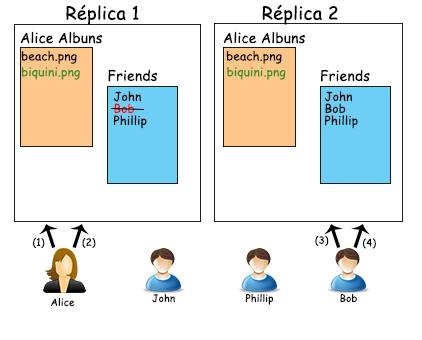
\includegraphics[scale=0.6]{Figure1}
\caption{Rede Social}
\label{fig:figure1.1}
\end{figure}

O desafio que este modelo apresenta, está representado na Figura \ref{fig:figure1.1}. Numa rede social em que cada utilizador tem vários álbuns e em que cada um tem fotografias as quais são partilhadas e visíveis pelos seus amigos e nas quais também podem ser feitos comentários. A possibilidade de ver estes álbuns, fotografias e fazer comentários sobre as mesmas apenas deve ser possível apenas a quem é amigo desse mesmo utilizador, de resto o sistema deve negar o acesso a páginas pessoas do utilizador a utilizadores arbitrários.

Neste caso a Alice tem um álbum que contém inicialmente uma foto \textit{"beach.png"} e tem três amigos o John, Philip e o Bob. No inicio do sistema qualquer um dos três amigos pode ir ver as fotos da Alice, ou seja, podem ter acesso à foto \textit{beach.png}  e fazer comentários na mesma. Todo este sistema está replicado ou seja, inicialmente temos a mesma informação tanto na réplica 1 como na réplica 2.
Depois de ter problemas com o Bob, a Alice decide que não quer que o Bob continue a ter acesso às suas fotos. Desta maneira ela vai remover o Bob da sua lista de amigos antes de fazer upload de uma novo foto, a qual não deseja que o Bob consiga ver, sendo por isto que ela removeu primeiro o Bob e apenas depois adicionou a nova foto.

Para a Alice interagir com o sistema, ela utiliza a réplica 1 que este caso é a que está mais perto dela. O que ela deseja é que primeiro que tudo seja removido o Bob dos amigos e apenas depois adicionada a foto, por isso ela faz essas operações segundo essa ordem na Réplica 1, sendo que na mesma não vão existir problemas devido sempre à existência de uma ordem parcial. Num sistema com garantias de consistência forte, nunca seria possível ao Bob aceder a novas fotos da Alice sem que ele fosse adicionado novamente à sua lista de amigos, algo que só seria possível se a Alice o assim desejasse. Contudo, num sistema replicado que só tenha garantias de consistência fraca, devido à não existência de uma ordem total, pode acontecer a réplica 2 receber a atualização de adição da foto \textit{biquini.png} antes da atualização de remover o Bob da lista de amigos da Alice. Isto vai permitir ao Bob, que vai estar ligado à réplica 2, a possibilidade de aceder à nova foto da Alice antes de chegar a mudança de políticas, ou seja, antes de chegar a atualização de lista de amigos da Alice.
Como podemos verificar a falta de ordenação total entre réplicas, faz com que possam existir alterações de dados e políticas fora de ordem, causando nestes casos fugas de informação sensível dos utilizadores. Para ser implementado um controlo de acessos sobre um sistema com consistência eventual, temos de ter então este problema em conta e manter ou respeitar ordenações entre políticas e subsequentes mudanças de dados e estas serem tidas em conta em todas as réplicas.

O artigo está organizado da seguinte forma: a secção 2 apresenta uma visão geral do funcionamento do sistema; na secção 3 discutimos com maior detalhe os vários problemas que se levantam e damos algumas introduções a como se resolvem; a secção 4 discute detalhes de implementação; a secção 5 apresenta a nossa avaliação experimental; o trabalho relacionado é abordado na secção 6 e finalmente, a secção 7 conclui o artigo e discute brevemente direções futuras para o trabalho apresentado.


%%%%%%%%%%%%%%%%%%%%%%%%%%%%%%%%%%%%%%%%%%%%%%%%%%%%%%%%%%%%%%%%%%%%%%%%%%%%%%%
\section{Vista Geral}\label{sec:vg}
%%%%%%%%%%%%%%%%%%%%%%%%%%%%%%%%%%%%%%%%%%%%%%%%%%%%%%%%%%%%%%%%%%%%%%%%%%%%%%%

Nesta secção apresentamos uma perspetiva geral sobre a arquitetura do sistema em que trabalhamos e no qual são demonstrados os desafios e as propostas inicias para os resolver. Neste caso vamos explicar primeiro o modelo formal do sistema, com a sua própria nomenclatura, as formas como as políticas e o sistemas de segurança devem funcionar atestando desta forma o seu correto funcionamento ou não em sistemas com consistências fraca.
Para isto ser possível vamos também definir semânticas de funcionamento correto para garantir que as mesmas são alcançadas para desta forma termos um objetivo concreto.

%%%%%%%%%%%%%%%%%%%%%%%%%%%%%%%%%%%%%%%%%%%%%%%%%%%%%%%%%%%%%%%%%%%%%%%%%%%%%%%
\subsection{Modelo Formal do Sistema} \label{mfs}
%%%%%%%%%%%%%%%%%%%%%%%%%%%%%%%%%%%%%%%%%%%%%%%%%%%%%%%%%%%%%%%%%%%%%%%%%%%%%%%

Para discutirmos o de funcionamento correto de um sistema de controlo de acessos com consistência fraca, precisamos de primeiro de tudo começar com um modelo formal de como a base do sistema está construida. 
O modelo base consiste num sistema de gestão de dados com consistência eventual. Este sistema tem um conjunto de dados que consiste em objetos, o $ \in $ \textit{Objects}. A estes objetos vão existir operações para conseguirmos modificar os mesmos que se designam op $ \in $ Op. Cada operação de modificação de dados vai ter também um objeto especifico que vai ser atualizado tendo desta forma um, \textit{target(op)} $ \in $ \textit{Objects}. As operações que podem ser executadas sobre os objetos são apenas duas, ou seja, nós apenas temos operações de leitura \textit{OpRead} ou operações de escrita em objetos, \textit{OpWrite}. Todas estas operações vão ser realizadas por um sujeito no nosso sistema, ou seja, cada operação vai formar um tuplo com um Sujeito s que fez uma operação (Op, s).
Neste sistema sabemos que vamos ter um determinado número de nós que vão fazer de \textit{host} aos nossos dados, sendo que assumimos que vamos ter replicação total, ou seja, que todos os objetos vão estar replicados em todos os nós.

As réplicas no nosso sistema são os nós que vão ter os dados replicados, sendo que as operações que os utilizadores vão fazer sobre as réplicas vão ser designadas como \textit{upstream operations}. Estas são as operações que o utilizador vai fazer sobre uma réplica especifica não se preocupando desta forma com as outras réplicas.

As réplicas vão depois sincronizar o seu estado enviando mensagens entre elas, ou seja, quando um utilizador faz uma operação, a mesma é executada na réplica a que ele estiver ligado. Posteriormente essa operação vai ser propagada para as outras réplicas havendo desta forma uma sincronização. A estas operações de envio de mensagens para outras réplicas para sincronizar chamamos de \textit{downstream operations}. As únicas operações que vão acontecer como \textit{downstream operations} são as de modificação, ou seja, \textit{OpWrite} dado que as operações de leitura apenas são aplicadas na réplica a quem o utilizador fez o pedido. Também aqui assumimos que estas \textit{downstream operations} têm garantias que eventualmente as mensagens chegam a cada outra réplica.

Cada réplica recebe das restantes \textit{downstream operations} que chegam numa ordem arbitrária. Neste caso estamos a assumir que os dados já têm propriedades para eventualmente, se pararem de existir operações de modificação, todas as réplicas acabarem com o mesmo valor, ou seja, vamos ter um sistema em que todas as réplicas vão ser iguais. Neste caso estamos a assumir que o nosso sistema de gestão de dados usa CRDTs (\textit{conflict-free replicated data types}) \cite{riak} \cite{zawirski2015write} \cite{shapiro2011conflict}  para garantir que os conflitos de escritas são resolvidos de forma idêntica em todas as réplicas. 

Também damos aqui uma noção de causalidade entre operações, em que a → b consiste em afirmar que 
a operação a ocorreu antes da operação b em alguma réplica R. Isto significa que alguém que esteja a utilizar a réplica R, viu o valor a antes de executar o valor b, ou seja a operação a estava visível na replica R quando a operação b foi executada.
Assumindo também que Cr$\langle$a$\rangle$ denota o tempo local no qual a operação a foi executada na réplica R. Não são feitas premissas sobre a relação de Cr$\langle$a$\rangle$ tempo global, mas é assumido que se a → b então Cr$\langle$a$\rangle$ < Cr$\langle$b$\rangle$.


%%%%%%%%%%%%%%%%%%%%%%%%%%%%%%%%%%%%%%%%%%%%%%%%%%%%%%%%%%%%%%%%%%%%%%%%%%%%%%%
\subsection{Politicas e Modelo de confiança} \label{p}
%%%%%%%%%%%%%%%%%%%%%%%%%%%%%%%%%%%%%%%%%%%%%%%%%%%%%%%%%%%%%%%%%%%%%%%%%%%%%%%

Quando nos estamos a referir a um sistema que queremos que seja seguro, temos de nos basear em algumas premissas que consideramos ser verdade, sendo isto que vamos discutir neste tópico. 

No nosso exemplo da rede social, cada uma das réplicas tem os dados de uma aplicação, sendo que essa aplicação pertence a uma entidade que vai necessitar de definir regras concretas para restringir as operações que sejam efetuadas por utilizadores. Continuando a nomenclatura definida anteriormente, sabemos que uma atribuição de direitos a um determinado sujeito vai resultar num triplo (r,s,o) $\in$ \textit{Rights X Subjects X Ojects}, ou seja, ficamos com um triplo contendo os direitos que um determinado utilizador tem sobre um determinado objeto. Quando nos referimos ao direito de uma operação ser executada estamos a referir-nos a r $\vdash$ Op, ou seja aquele direto r permite a operação Op. Quando damos direitos (r,s,o) sabemos que o mesmo permite uma operação se e só se (r,s,o) $\models$ (op, s') iff r $\vdash$ op, target(op) = o e s = s'. 

Em relação às políticas sabemos que vão estar contidas em cada réplica, sendo que desta forma funcionam de forma semelhante ao dados que falamos anteriormente. Quando é feito uma modificação de direitos o ficheiro de políticas é alterado numa das réplicas e depois vai existir uma troca de mensagens para essa informação chegar a todas as réplicas e todas as políticas serem sincronizadas.

\begin{figure}[h]
\centering
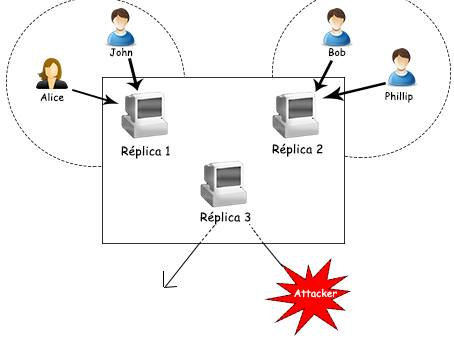
\includegraphics[scale=0.6]{Figure2}
\caption{Rede de Confiança no Sistema}
\label{fig:figure2.1}
\end{figure}

Em relação ao grau de confiança em relação às réplicas neste sistema de gestão de dados, assumimos que todas as \textit{upstream operations} (operações invocadas pelos utilizadores) vão ser verificadas na réplica ao qual esse utilizador está ligado, de forma a aferir se o mesmo tem permissões para efetuar as modificações que deseja. Esta verificação vai se apenas feita em \textit{upstream operations}, sendo que \textit{downstream operations} são realizadas sem a necessidade de qualquer tipo de verificação em relação às políticas atuais. Estas nossas premissas vão de acordo com o que existe atualmente dado que partimos do principio que uma aplicação pertence a uma organização e que a mesma tem controlo sobre todas as réplicas, ou seja, todas as réplicas estão dentro de um sistema confiável.

A Figura \ref{fig:figure2.1} mostra este nosso sistema, em que todas as réplicas R1, R2 e R3 podem comunicar diretamente sem necessitarem de verificar as permissões das operações, funcionando como que num género de caixa negra em que é como se assumíssemos que ali apenas estava um servidor, ficando tudo dentro do mesmo nível de segurança (se é aceite numa réplica, por sabermos que todas são mutuamente seguras assumimos que também vai ser aceite em todas as outra). Quando um utilizador se autentica no sistema, o mesmo vai entrar temporariamente dentro do ambiente protegido, sendo que depois quando quiser fazer algum tipo de operações sobre o sistema (\textit{upstream operations}), estas vão ser verificadas pela réplica à qual ele está ligado, neste exemplo da Figura \ref{fig:figure2.1} a Alice iria tentar fazer uma modificação mas só o conseguiria se na réplica 1 lhe fosse permitido na lista dos seus direitos.

Desta forma qualquer utilizador não autenticado iria ficar sempre de fora do ambiente protegido sendo que mesmo se fosse um utilizador autenticado mas tentasse fazer escritas ou leituras que não devia, as mesmas seriam rejeitadas.

%%%%%%%%%%%%%%%%%%%%%%%%%%%%%%%%%%%%%%%%%%%%%%%%%%%%%%%%%%%%%%%%%%%%%%%%%%%%%%%
\section{Como o Controlo de Acessos deve Funcionar e Desafios}\label{sec:challenges}
%%%%%%%%%%%%%%%%%%%%%%%%%%%%%%%%%%%%%%%%%%%%%%%%%%%%%%%%%%%%%%%%%%%%%%%%%%%%%%%

Para um sistema de controlo de acessos estar correto, isto implica que vai fazer as suas políticas de segurança serem seguidas em todas as réplicas. Quando estamos a falar de um sistema com consistência forte, sabemos que uma operação Op realizada por um utilizador s, apenas vai ser aceite se as políticas de segurança o permitirem ou seja se existir uma permissão (r,s,o) $\models$ (op,s). Num sistema com consistência forte, sabemos que para a operação op ser aceite, precisa de ter havido antes a ação de dar permissões sobre a mesma, ou seja, precisamos que (r,s,o) → (op,s). 

Num sistema fortemente consistente é possível falarmos sobre a política de controlo de acessos atual, isto pela existência de uma ordem global de operações no sistema. Desta forma para sabermos a política de controlo atual num sistema fortemente consistente, apenas precisamos de pegar no estado inicial da política e aplicar todas as operações op por ordem.

Já num sistema com consistência fraca, não existe ordem total entre operações. Em cada réplica existe uma ordem pela qual as operações são executadas, mas esta ordem pode variar de réplica para réplica. Sem adicionarmos nenhuma forma de sincronização entre réplicas, ficamos apenas com a possibilidade de nos referirmos ao estado da cópia local da política de controlo de acessos.

As operações sobre os dados podem depender da modificação de políticas de duas maneiras diferentes:

1) Uma operação é válida pois houve uma mudança de políticas que o permite:
\\
\begin{center}
(r,s,o) → (OpWrite, s) $\wedge$ (r,s,o) $\models$ (OpWrite, s)
\end{center}
2) Uma modificação de política protege a modificação de um objeto removendo o acesso para um utilizador especifico:
\\
\begin{center}
(r, s1, o) → (OpWrite, s2) and (r, s1, o) $\not\models$ (OpRead, s1)
\end{center}


\begin{figure}[h]
\centering
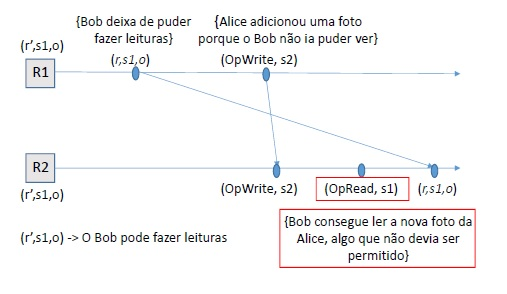
\includegraphics[scale=0.6]{Figure31}
\caption{Violação de políticas de acesso caso 1}
\label{fig:figure3.1}
\end{figure}

Na Figura \ref{fig:figure3.1} apresentamos a situação descrita anteriormente no ponto 1. Assumindo que as políticas de segurança nas réplicas permitem a leitura do objeto o pela utilizador s1, (r',s1,o) $\models$ (OpRead, s1). Como podemos ver na imagem um a entidade autorizada depois muda as políticas de segurança na réplica 1 para (r,s1,o) sendo que na mesma réplica e após algum tempo uma entidade s2 faz uma escrita de um objecto (OpWrite, s2).

Como podemos ver na réplica na figura 3.1, por não existir uma ordem total entre réplicas, a réplica R2 pode receber as operações fora de ordem. Desta maneira pode receber primeiro a operação em que vai existir uma alteração de dados numa altura em que ainda é possível à entidade s1 ver essa informação, dado que nessa réplica (OpWrite, s2, o) → (OpRead, s1) → (r,s1,o). Isto vai ser uma violação da política de segurança e deve ser considerado um funcionamento incorreto da política de controlo. 

\begin{figure}[h]
\centering
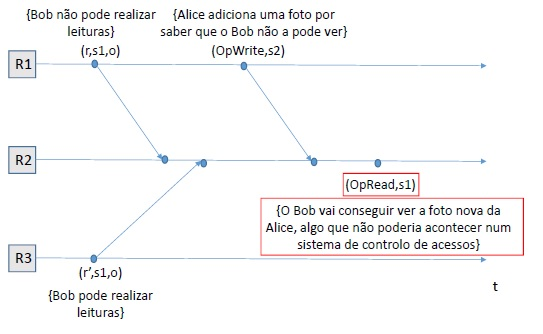
\includegraphics[scale=0.6]{Figure32}
\caption{Violação de políticas de acesso caso 2}
\label{fig:figure3.2}
\end{figure}

Na Figura \ref{fig:figure3.2} também está representado outro dos problemas existentes. Anteriormente foi explicado que tem de existir uma ordem entre as operações, mas e se acontecerem múltiplas escritas concorrentes de políticas?

Estão representadas na figura \ref{fig:figure3.2} três réplicas que têm um estado inicial igual. Na réplica R1 é feita uma alteração de políticas consistindo em (r,s1,o) e ao mesmo tempo é feita uma alteração de políticas consistindo em (r',s1,o). Sabendo que a ordem à qual as operações podem chegar a R2 é arbitrária, ficamos com a possibilidade da réplica R2 receber primeiro a alteração de políticas de R1 e depois a de R3, e apenas depois uma escrita vinda de R1 com uma leitura feita de seguida em R2 pelo utilizador s1.

O problema é assumindo que (r,s1,o) não permite a leitura ao utilizador s1, isso significa que na réplica R1 foi visível quando foi feita a operação (OpWrite, s2) que não existia essa permissão. Ou seja, criando uma analogia com o nosso exemplo anterior a Alice iria estar a remover o Bob e de seguida a adicionar uma foto, pois ela viu na sua réplica que o Bob estava realmente removido. Mas se na réplica R3 for feito concorrentemente uma modificação de políticas (r',s1,o) em que r' permite a s1 que faça operações de leitura podemos ter o caso de na réplica 2 quando ambas as mudanças convergem, elas ficarem sobre uma ordem que vá permitir a fuga de informação. Neste caso iria ser feita uma alteração na réplica 3 a dizer que Bob poderia ver as fotos e desta forma seria possível ao Bob ver as fotos na réplica 2 se as operações de remoção de permissão de leitura chegassem antes das de adição de permissão de leitura (r,s1,o) → (r',s1,o), não respeitando a privacidade requisitada na réplica 1.

%%%%%%%%%%%%%%%%%%%%%%%%%%%%%%%%%%%%%%%%%%%%%%%%%%%%%%%%%%%%%%%%%%%%%%%%%%%%%%%
\subsection{Semanticas} \label{semantics}
%%%%%%%%%%%%%%%%%%%%%%%%%%%%%%%%%%%%%%%%%%%%%%%%%%%%%%%%%%%%%%%%%%%%%%%%%%%%%%%

Neste caso o controlo de consistência entre réplicas é apenas eventual, sendo que não existem garantias de quando as atualizações vão ser realizadas em todas as réplicas nem com que ordem, sendo possível estados temporariamente inconsistentes.
No caso do controlo de acessos, como já falamos, isto pode levantar problemas. 
Sendo que estamos a olhar para sistemas geo-replicados, sabemos que cada réplica é apenas uma cópia da outra e não vai ter restrições próprias de controlo de acesso, ou seja, todas as réplicas vão conseguir propagar e ler todas as alterações que foram feitas. Com isto podemos adotar um sistema de confiança mútua entre todas estas réplicas em que podemos assumir uma caixa negra, assumindo que todas estas réplicas funcionam como um apenas servidor.
Para vermos como funciona temos 4 operações que vamos descrever. Estas operações são mudanças nas políticas de controlo de acessos, são elas: Permitir Leituras; Permitir Escritas; Revogar Leitura; Revogar Escrita.


\paragraph{\textbf{\textit{•Permitir Leituras}}}

No caso de dar permissões de leitura a um utilizador que ainda não as tinhas, dado que sabemos que eventualmente todos os servidores vão saber que o utilizador tem aquelas permissões e vão dar acesso aos seus dados. O único problema que poderia haver seria um utilizador dar permissões e depois fazer uma modificação, esperando que o outro o pudesse ver, mas como sabemos eventualmente vai ser possível, mesmo que a atualização de dados se processe antes do controlo de acessos, desta forma nunca criando inconsistência.

\paragraph{\textbf{\textit{•Permitir Escritas: }}}
Neste caso pode existir a tentativa de dar as permissões a um utilizador. Sabendo que a propagação vai ser eventual sabemos que eventualmente todas as réplicas vão saber as permissões desse mesmo utilizador. Nunca vai ser problemático se optarmos por usar o modelo de aceitar e rejeitar atualizações segundo o modelo de confiança mútua entre os servidores. Ou seja, desta forma, se um cliente ficar com permissões de escrita e o seu servidor souber que as tem, ele vai marcar na mensagem da modificação que permitiu a atualização.
\\
\\
\textbf{Escritas quando aceites por uma replica devem ser assinadas pela mesma, e apenas depois enviadas para as outras replicas, desta forma garantindo que vão ser aceites em todas as replicas.}


\paragraph{\textbf{\textit{•Revogar Leitura}}}

No caso em que deixamos de permitir leituras vamos ter o problema da mobilidade do utilizador e também da ordenação de operações. Isto porque o mesmo pode tentar mudar de réplica para ler da réplica que ainda lhe permite ver as novas atualizações. Desta forma sabemos que se este utilizador se mantiver sempre ligado à mesma réplica apenas teremos o problema de se por exemplo uma nova modificação vier para a nossa réplica antes da remoção de permissões de leitura, mesmo que na origem tenham sido feitas primeiro as operações de tirar permissão de leitura e depois fazer a atualização. Com isto temos mais 2 pontos chave:
\\
\\
\textbf{O utilizador tem de ter uma baixa capacidade de mudar de réplica por sua própria vontade, sem ser quando uma réplica fica indisponível.}
\\
\textbf{As operações de atualização de dados e de revogação de permissões têm de ter uma ordenação causal para desta forma não permitir ver atualizações já depois de permissões terem sido removidas.
}

\paragraph{\textbf{\textit{•Revogar Escrita}}}

Quando se nega uma escrita continuamos a ter o problema descrito anteriormente, em que o cliente pode mudar de réplicas para onde ainda tem permissões.


%%%%%%%%%%%%%%%%%%%%%%%%%%%%%%%%%%%%%%%%%%%%%%%%%%%%%%%%%%%%%%%%%%%%%%%%%%%%%%%
\section{Detalhes de Implementação}\label{sec:implementacao}
%%%%%%%%%%%%%%%%%%%%%%%%%%%%%%%%%%%%%%%%%%%%%%%%%%%%%%%%%%%%%%%%%%%%%%%%%%%%%%%

Como foi explicado na secção anterior, existiam dois problemas para resolver. O facto de poderem existir fugas de informação e o que acontece quando existem múltiplas modificações à política de controlo de forma concorrente.

Para isto foi usado um sistema de gestão de dados distribuído que funciona com consistência eventual. Toda a gestão dos dados desse sistema é atingida pelo uso de CRDT's.

Afim de serem implementadas políticas de controlo de acesso foram desenvolvidos novos CRDTs com controlo de acessos. Estes CRDTs têm as mesmas propriedades que os outros, sendo também possível detetar quando são feitas escritas concorrentes nos mesmos. Todos estes CRDTs têm duas operações importantes para este contexto, a função de \textit{generatedownstream}, que gera uma mensagem para as outras réplicas onde dentro dessa mensagem vai o valor das políticas atuais, e a função \textit{update}, que é chamada sempre que uma réplica recebe uma operação de \textit{downstream}, neste caso um dos argumentos também é o valor das políticas atual e o valor das políticas que vem na mensagem do \textit{generatedownstream}. Desta forma é possível saber se existem alterações entre a execução do \textit{downstream} e os \textit{updates}, detetando desta forma operações concorrentes. 
Se existem operações concorrentes adicionamos as permissões a uma lista, podendo neste caso haver várias permissões para o mesmo utilizador ([$\lbrace$Bob, "read"$\rbrace$ ,$\lbrace$Bob,"read,write"$\rbrace$]). Já se ambas as políticas são iguais isto significa que não existiram operações concorrentes e podemos apenas atualizar as permissões desse utilizador.

Em relação aos problemas encontrados anteriormente, em primeiro lugar a necessidade de não haver perda de informação das políticas quando são realizadas operações de escrita sobre as mesmas de forma concorrente. Quando existem modificações concorrentes a representação de cada uma delas vai dar-nos o conhecimento sobre o que cada réplica permite, sendo que o objetivo é existir uma defesa contra a possibilidade de serem feitas posteriormente edições ou leituras sobre os dados que deveriam estar protegidos. No caso da Alice e do Bob dado como exemplo anteriormente seria necessário registar na réplica intermédia que estavam a existir operações concorrentes e que as mesmas tinhas de ser juntas de forma a ser possível interpretar o que se passa em cada uma das réplicas. Tendo as várias políticas das várias réplicas é assim possível optar por um caminho mais seguro, em que para serem calculadas as permissões, vamos verificar o mínimo entre as operações de modificação de políticas concorrentes que existiram. Na nossa implementação iríamos desta forma usar as múltiplas permissões guardadas quando eram detetadas modificações concorrentes e quando era pedido para saber o valor de permissão do utilizador era calculado um mínimo.

Outro dos problemas era a falta de um ordenação das operações, sendo possível operações de escrita realizadas numa réplica a seguir a uma edição de políticas, ser vista de forma inversa noutras réplicas criando desta forma a possibilidade de termos fuga de informação sensível. Podia ter sido usada como solução o uso de causalidade entre operações segundo os relógios de Lamport [BIBLIOGRAFIA]. Contudo isto não foi o aplicado, sendo que desta forma era resolvido o desafio de desordenação de operações, mas teria de existir uma ligação entre cada CRDT de políticas e cada CRDT de dados. A solução adotada foi juntar ambos, ou seja, as políticas de controlo de acesso estarem dentro do objeto referido. Esta solução acaba por aumentar a complexidade devido a ser necessário implementar as políticas de controlo de acesso para cada CRDT. Desta forma, quando é realizada uma operação de escrita as políticas que estavam em uso durante essa mesma operação vão acompanhar a mensagem. Quando chegam a outra réplica estas políticas são adicionadas às políticas atuais e é calculado um mínimo, sendo que desta forma se numa réplica R1 não for permitido o Bob ver uma alteração e de seguida nessa mesma réplica for feita uma mudança de um objeto, é possível saber com certezas que o Bob não vai conseguir ver essa alteração em nenhuma das réplicas devido ao cálculo dos mínimos.

%%%%%%%%%%%%%%%%%%%%%%%%%%%%%%%%%%%%%%%%%%%%%%%%%%%%%%%%%%%%%%%%%%%%%%%%%%%%%%%
\section{Avaliação}\label{sec:av}
%%%%%%%%%%%%%%%%%%%%%%%%%%%%%%%%%%%%%%%%%%%%%%%%%%%%%%%%%%%%%%%%%%%%%%%%%%%%%%%

%%%%%%%%%%%%%%%%%%%%%%%%%%%%%%%%%%%%%%%%%%%%%%%%%%%%%%%%%%%%%%%%%%%%%%%%%%%%%%%
\section{Trabalho Relacionado}\label{sec:related work}
%%%%%%%%%%%%%%%%%%%%%%%%%%%%%%%%%%%%%%%%%%%%%%%%%%%%%%%%%%%%%%%%%%%%%%%%%%%%%%%

%%%%%%%%%%%%%%%%%%%%%%%%%%%%%%%%%%%%%%%%%%%%%%%%%%%%%%%%%%%%%%%%%%%%%%%%%%%%%%%
\section{Trabalho Futuro}\label{sec:future work}
%%%%%%%%%%%%%%%%%%%%%%%%%%%%%%%%%%%%%%%%%%%%%%%%%%%%%%%%%%%%%%%%%%%%%%%%%%%%%%%

Este artigo de investigação consiste no primeiro passo para providenciar controlo de acessos ao sistema em que estamos a trabalhar, Legion \cite{mastersthesis}. O mesmo procura enriquecer a forma como são vistas as aplicações web, oferecendo também direta interação direta entre clientes para aumentar a disponibilidade e latência de pedidos, isto tudo criando uma rede de \textit{peer-to-peer} entre clientes.

Neste caso este artigo vai de encontro em primeiro que tudo estabelecermos este acesso de controlo na componente centralizada quem tem de ser usada para ser mantido o estado do sistema e dar uma base confiável. 

O passo seguinte será estender estas políticas de acesso de controlo para conseguirmos fazer o mesmo com clientes que vão consistir em réplicas parciais do sistema, acrescentando complexidade à nossa solução neste artigo e também devido ao facto de os clientes não poderem ser admitidos como confiáveis, ou seja, enquanto neste nosso artigo admitimos que as mensagens passadas entre servidores são sempre aceites pois se uma réplica aceita uma atualização sabemos que ela é confiável e a devemos respeitar, já no novo modelo com os clientes não o podemos fazer, não sendo possível desta forma propagar operações da mesma forma.

%%%%%%%%%%%%%%%%%%%%%%%%%%%%%%%%%%%%%%%%%%%%%%%%%%%%%%%%%%%%%%%%%%%%%%%%%%%%%%%
\bibliographystyle{splncs03}
\bibliography{paper}
%%%%%%%%%%%%%%%%%%%%%%%%%%%%%%%%%%%%%%%%%%%%%%%%%%%%%%%%%%%%%%%%%%%%%%%%%%%%%%%

\end{document}
